\documentclass[a4paper,12pt]{book}
\usepackage{graphicx}
\usepackage{float}
\usepackage[T1]{fontenc}
\usepackage{hyperref}
\usepackage{adjustbox}
\graphicspath{ {./images/} }
\pagenumbering{gobble}
\begin{document}

\author{Miłosz Wojciechowski}
\title{Telemetry extractor manual}
\date{\today\\ v0.4}


\maketitle
\pagebreak
\pagenumbering{arabic}
\renewcommand{\labelenumii}{\arabic{enumi}.\arabic{enumii}}
\tableofcontents
\chapter{Introduction}
\section{GoPro video types}
File structure of GoPro Max videos:\\	
GoPro Max creates 3 types of files during recording, in 360 mode we get:
	\begin{itemize}
		\item .360 file (main video file)
		\item .THM file (thumbnail file)
		\item .LRV file (low-res video file)\\
	\end{itemize}
	In HERO mode (traditional video in 1080p or 1440p) we get:
	\begin{itemize}
		\item .MP4 file (main video file)
		\item .THM file (thumbnail file)\\
	\end{itemize}
	These files always appear after recording a classical video or a Time Lapse.\\
	
\section{How to record a video}
\begin{enumerate}
	\item Record a video with your GoPro camera (traditional video in HERO or 360 mode, Time Lapse in HERO or 360 mode). How to use GoPro MAX camera is described in the GoPro MAX manual available under \href{https://gopro.com/content/dam/help/max/manuals/MAX_UM_ENG_REVB.pdf}{this link}. Make sure that you have turned on GPS function otherwise video won't have telemetry data:
	\begin{figure}[H]
		\centering
		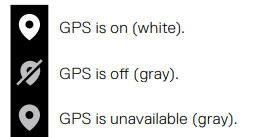
\includegraphics{GoPro_manual_fragment}
		\caption{GoPro Max manual fragment.}
	\end{figure}
	If GPS is off, swipe down to access the Dashboard and Preferences. Click on the Preferences, find option Regional and there turn the GPS On.\\
\end{enumerate}
\section{Export camera recordings}
\begin{enumerate}
\item Turn on your GoPro camera.
\item Open your GoPro MAX side panel and connect it to your computer using USB 2.0 to USB-c cable included in a camera set. Information as below should display on the screen:
\begin{figure}[H]
	\centering
	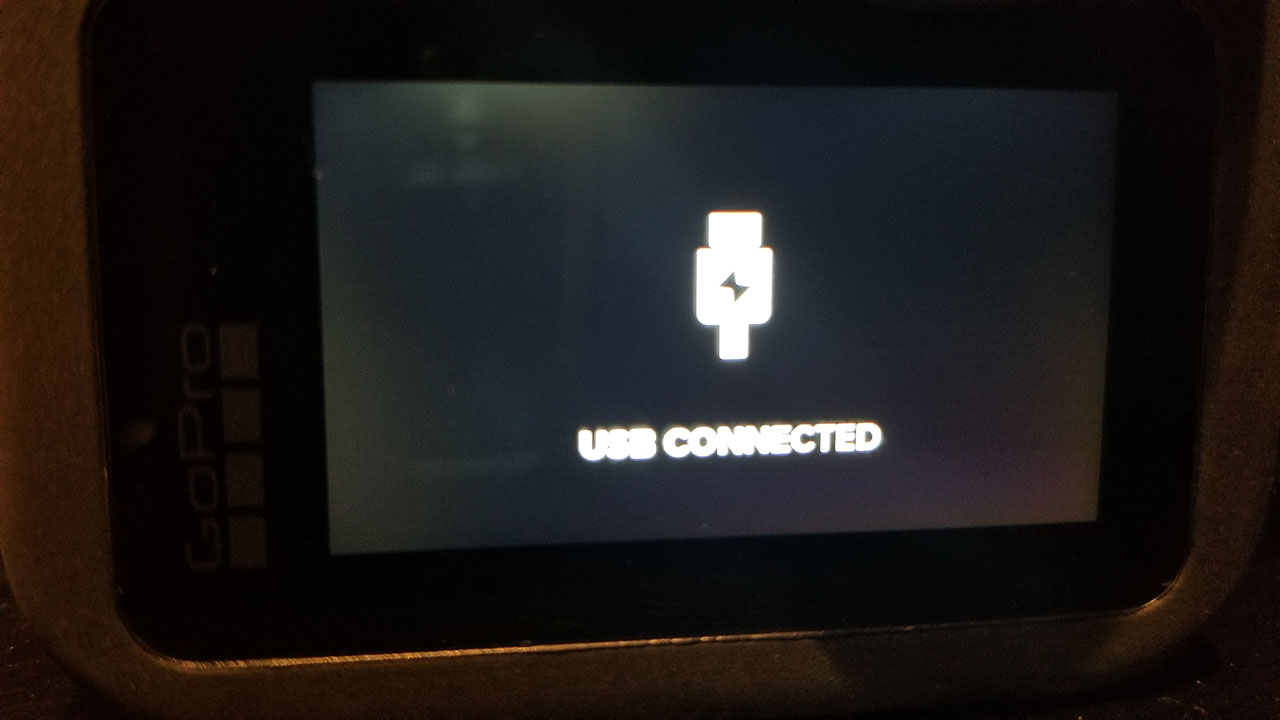
\includegraphics{camera_connected}
	\caption{Successfully connected camera.}
\end{figure} 

\item Now find your connected GoPro camera and navigate through directories:\\

$\textit{GoPro MAX > GoPro MTP Client Disk Volume > DCIM > 100GOPRO}$	\\

Final path should look like this:

\textit{GoPro MAX/GoPro MTP Client Disk Volume/DCIM/100GOPRO}	
\begin{figure}[H]
	\centering
	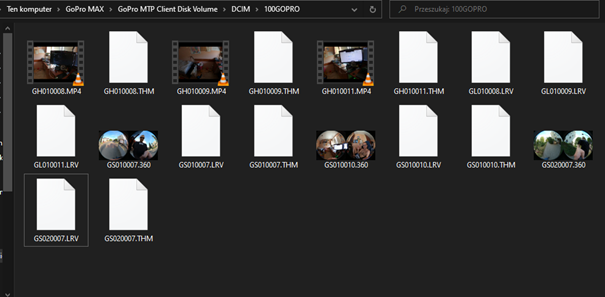
\includegraphics{recording_location}
	\caption{Video files location.}
\end{figure}
\hfill
\item 360 videos’ names and their LRV versions start with GS e.g. GS020007.360, GS020007.LRV.\\

Regular videos’ and their LRV versions’ names start with GH for the former and with GL for the latter e.g. GH010008.MP4, GL010008.LRV. \\
\end{enumerate}

\chapter{Install environment and Git}
\section{Install Git}
\begin{enumerate}
	\item Download Git installer from \url{https://gitforwindows.org} and run it.
	\item \begin{minipage}[t]{\linewidth}
		\raggedright
		\adjustbox{valign=t}{%
			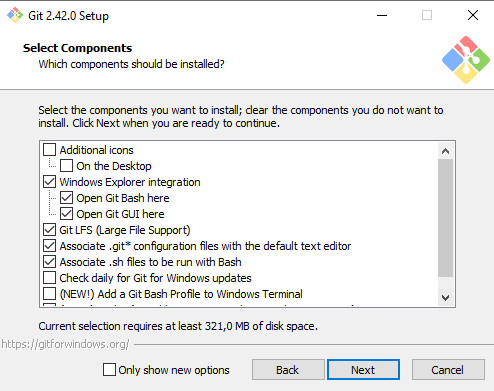
\includegraphics[width=.8\linewidth]{git_install1}%
		}		
		\medskip	
	\end{minipage}
	Select components as seen in the picture above.
	
	\item \begin{minipage}[t]{\linewidth}
		\raggedright
		\adjustbox{valign=t}{%
			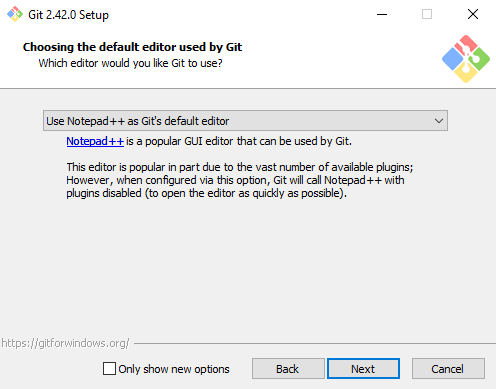
\includegraphics[width=.8\linewidth]{git_install2}%
		}		
		\medskip	
	\end{minipage}
	Choose default editor for Git, I recommend Notepad++ if you don't have it download it from here: \url{https://notepad-plus-plus.org/downloads/}. Install the newest version, you don't have to change anything during installation, just accept and install.
	\item \begin{minipage}[t]{\linewidth}
		\raggedright
		\adjustbox{valign=t}{%
			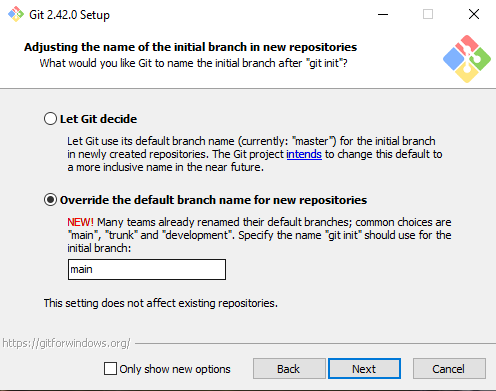
\includegraphics[width=.8\linewidth]{git_install3}%
		}		
		\medskip	
	\end{minipage}
	Select to override since many guides now use the word "main" not "master" for main branch
	\item \begin{minipage}[t]{\linewidth}
		\raggedright
		\adjustbox{valign=t}{%
			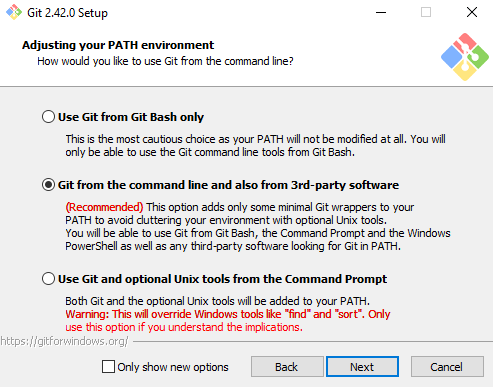
\includegraphics[width=.8\linewidth]{git_install4}%
		}		
		\medskip	
	\end{minipage}
	\item \begin{minipage}[t]{\linewidth}
		\raggedright
		\adjustbox{valign=t}{%
			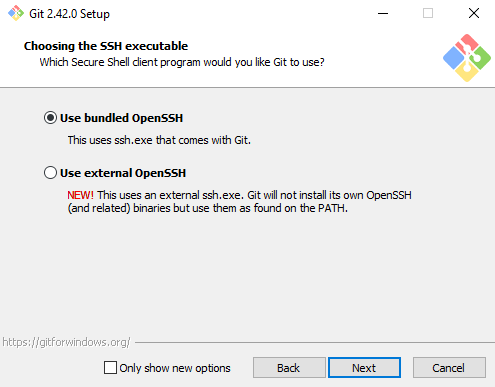
\includegraphics[width=.8\linewidth]{git_install5}%
		}		
		\medskip	
	\end{minipage}
	Choose option to use ssh that comes with Git.
	\item Go through all next appearing windows and change nothing in them. At the end click "Install".
\end{enumerate}
\pagebreak
\section{Install node js}
\begin{enumerate}
	\item Go to \url{https://nodejs.org/en} and download recommended version and run the installer.
	\begin{figure}[H]
		\centering
		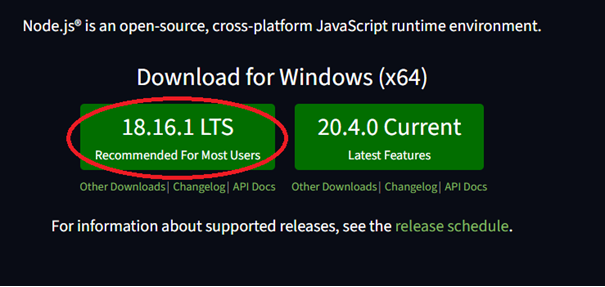
\includegraphics{nodejs_install}
		\caption{Nodejs website fragment.}
	\end{figure}
	\item \begin{minipage}[t]{\linewidth}
		\raggedright
		\adjustbox{valign=t}{%
			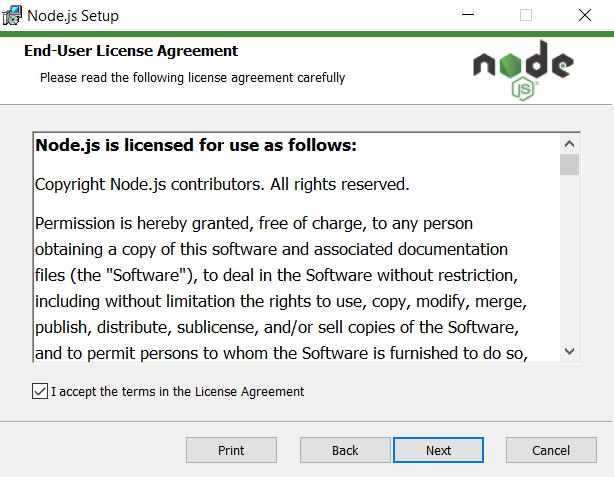
\includegraphics[width=.8\linewidth]{node_install0}%
		}		
		\medskip	
	\end{minipage}
	Accept user agreement
	\item \begin{minipage}[t]{\linewidth}
		\raggedright
		\adjustbox{valign=t}{%
			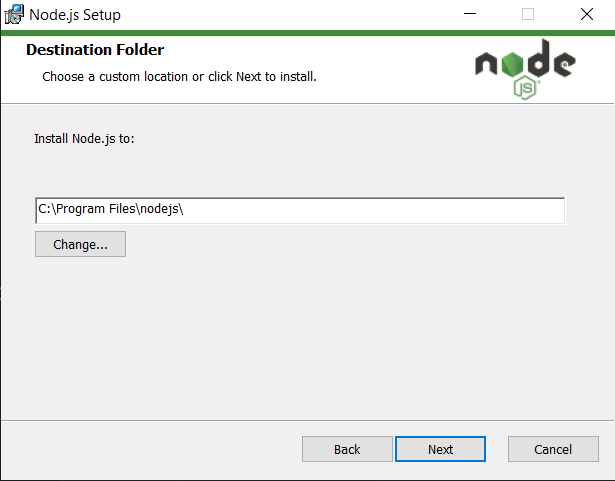
\includegraphics[width=.8\linewidth]{node_install1}%
		}		
		\medskip	
	\end{minipage}
	Choose location, default one is sufficient.
	\item \begin{minipage}[t]{\linewidth}
		\raggedright
		\adjustbox{valign=t}{%
			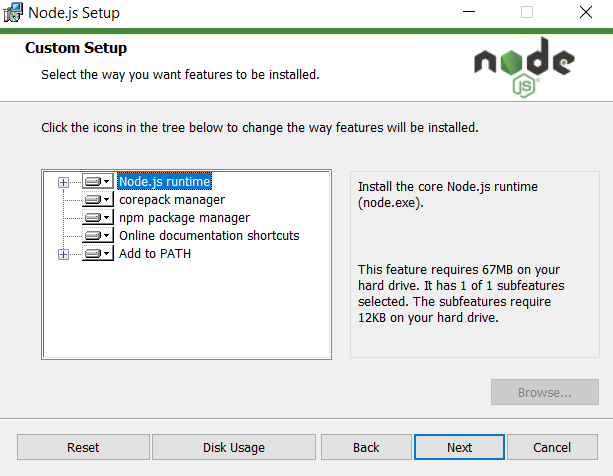
\includegraphics[width=.8\linewidth]{node_install2}%
		}		
		\medskip	
	\end{minipage}
	Do not change anything, install everything as it is.
	\item \begin{minipage}[t]{\linewidth}
		\raggedright
		\adjustbox{valign=t}{%
			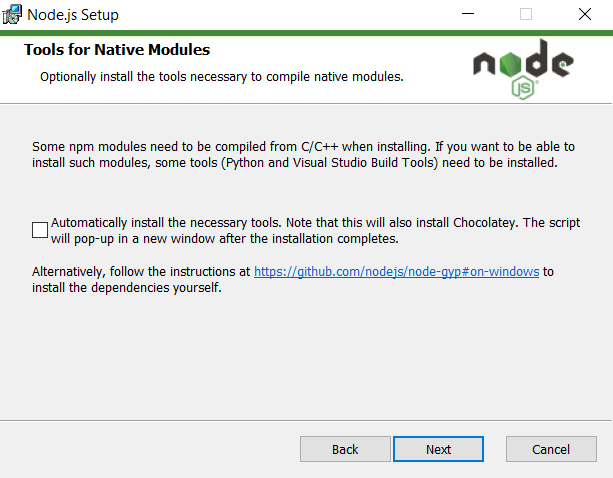
\includegraphics[width=.8\linewidth]{node_install3}%
		}		
		\medskip	
	\end{minipage}
	You do not need to install extra tools to run telemetry extractor.
	\item \begin{minipage}[t]{\linewidth}
		\raggedright
		\adjustbox{valign=t}{%
			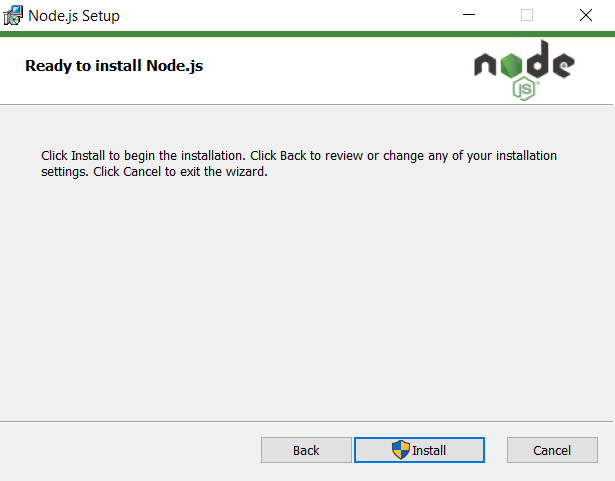
\includegraphics[width=.8\linewidth]{node_install4}%
		}		
		\medskip	
	\end{minipage}
	Click Install to begin installation
	\pagebreak
	\item To check if installed correctly simply open Command Prompt by typing “cmd” in the Start Menu and write “node”, if everything was done properly version of node should appear.
	\begin{figure}[H]
		\centering
		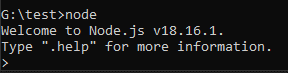
\includegraphics{node_confirmation}
		\caption{Command Prompt fragment confirming proper installation of Nodejs.}
	\end{figure}
\end{enumerate}
	
\chapter{Run Telemetry-extractor}
\section{Download program and dependencies from Git}
\begin{enumerate}
	\item Download main repository: \url{https://github.com/miloszwojciechowski/Open-vslam-project} and extract it in directory of your choice.
	\item \begin{minipage}[t]{\linewidth}
		\raggedright
		\adjustbox{valign=t}{%
			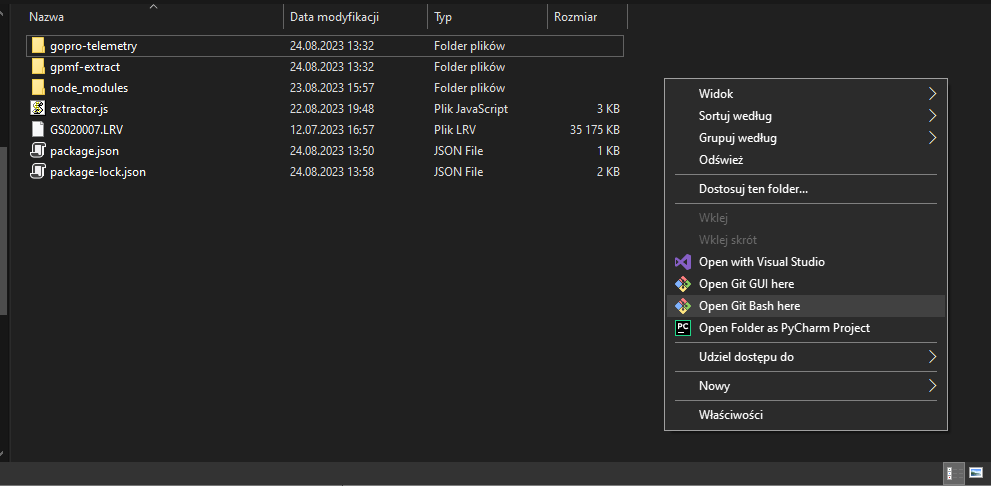
\includegraphics[width=.8\linewidth]{run1}%
		}		
		\medskip	
	\end{minipage}
	Go to folder where the repository has been extracted and right click on free space and click Open Git Bash here.
	\item \begin{minipage}[t]{\linewidth}
		\raggedright
		\adjustbox{valign=t}{%
			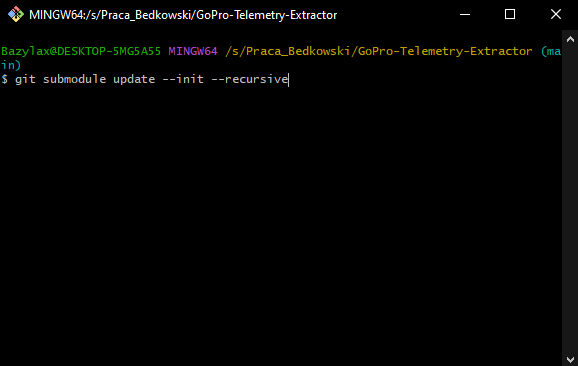
\includegraphics[width=.8\linewidth]{run2}%
		}		
		\medskip	
	\end{minipage}
	Now write the following command: \textit{git submodule update \texttt{-{}-}init \texttt{-{}-}recursive} or copy it from here and right click on the Bash and click Paste. And lastly run the command. \\
	If you use Git for the first time, information will pop that you need to identify yourself, follow the instructions to log with your GitHub account.\\
	Fulfilling this step will download \href{https://github.com/JuanIrache/gopro-telemetry}{gopro-telemetry} and \href{https://github.com/JuanIrache/gpmf-extract}{gpmf-extract}
	\item You can close git bash and open Command Prompt by typing cmd in Windows Start Menu.
	\item Choose the disc on which you have telemetry extractor by writing disc letter followed by colon e.g. D:
	\item Move to telemetry extractor directory by typing "cd" followed by the name of desired directory e.g cd GoPro-Telemetry-Extractor.
	\item From there move to both: gopro-telemetry and gpmf-extract (again by using cd <directory name>, if you want to go to previous directory type "cd..") and in both directories write \textit{npm install} to install libraries.
\end{enumerate}

\section{Run the program}
\begin{enumerate}
	\item In command prompt go to GoPro-Telemetry-Extractor location (the one with extractor.js file) 
	\item Copy to this directory a video file you want to extract telemetry data from (if it's just telemetry I suggest using .LRV file since it will work much faster)
	\item Run the program by writing “node extractor.js <your video file name> e.g. "node extractor.js GS020007.LRV". Telemetry .csv file will appear in the same location as extractor.js file.
\end{enumerate}
 
\end{document}